% Chapter 1

\chapter{Introduction} % Main chapter title

\label{Chapter1} % For referencing the chapter elsewhere, use \ref{Chapter1} 

\lhead{Chapter 1. \emph{Introduction}} % This is for the header on each page - perhaps a shortened title

%----------------------------------------------------------------------------------------

Imagine you are at the library, studying, and you decide to take a little break. You start observing your friend sitting next to you, and he is reading a book. Suddenly he looks at the girl sitting across you. 'Automatic reflex', you may think, if you think about it at all. But then he looks at her a second time, and a third, and a fourth. Now you are thinking 'What is he doing?' 'Who is she?', and you may even look at the girl yourself.  

Why do we behave like that?  We don't pay attention when unusual things happen once, but we become curious when an unusual thing happens several times.

\label{curiosity}
Curiosity is defined as “a strong desire to know and learn something" and as an “unusual or interesting object or fact" \cite{oxford}. Curiosity means giving importance to what you do not recognize, and wanting to learn about it. This process is inherent in humans and other animals. As toddlers, we are curious about anything new, and we learn by asking questions like 'What is that?' or 'Why is it like that?'. We actively want to know about new and strange things and we want to learn about them, to be able to recognize them the next time.

The process of being curious relies on identifying novel stimuli that are “different from anything known before; new, interesting and often seeming slightly strange” \label{novel} \cite{Pimentel2014} and being able to learn from them, while ignoring stimuli that are already known or seem uninteresting. Therefore, curiosity can imply a desire of learning a new stimuli when it is considered strange and interesting.

In the field of Artificial Intelligence, Machine Learning is the branch that deals with the design and study of mathematical systems that can learn from data. The methods used in Machine Learning have been applied to the field of robotics, enabling robots to learn new abilities. Traditional methods in Machine Learning are based on passive learning. In such learnings, the robot system would create a model from the data in the training phase, and then it would predict a classification for new data in the test phase. However, in most of these methods, inputs are being introduced and analyzed by a human operating the system, therefore, the system is simply a computational tool. Classification is pre-conditioned by the data in the training system, the knowledge base, and it is only be expanded if the human operator includes more data in the training set and the system can relearn. 

In \emph{active learning}, the system itself is an actor in the learning process. The system can understand and decide what is relevant and what is unknown, and it is intrinsically motivated to explore the areas of the learning space that it does not know, ask the user about them and add new data to its knowledge base. Thus, the learning process is directed by the system and is continuous. The system can learn autonomously and interact with the humans to ask for more information if it needs to. Interactive robots are also perceived as more intelligent by humans \cite{Cakmak2010}.

For this purpose, in the development of Machine Learning, this process of curiosity is critical. It constitutes an important component for the effective and long-term operation of intelligent robot systems allowing computationally efficient, unsupervised and incremental exploration and learning of new skills and environments \cite{Nehmzow2013}. This ability means a huge step in their autonomy and learning habits, making them process information more like humans. This is key because it brings us closer to the "holy grail of Artificial Intelligence: general purpose human level intelligence equivalence"\cite{Brooks1990}. 

This Thesis presents a system that allows a human-interactive robot to be able to actively want to learn about novel stimuli presented to it, via a visual system, expanding its knowledge base. The system will be able to detect novel stimuli using machine learning algorithms, analyzing if a stimuli is interesting and different than anything seen before. When a novel stimuli is detected the system learns the data and adds it to its knowledge base. When the stimuli is considered known or not interesting, the system will ignore it. \footnote{The definitions of \emph{new}, \emph{interesting} and \emph{strange} will be further developed in the introduction of Chapter \ref{Chapter2}.}

The general learning performance of the system is based on ignoring perceptions that are already known, and highlighting novel stimulus.  This concept is based of what is called habituation, and is inspired on biological systems. Habituation is a “type of non-associative learning used to describe the behavioral phenomenon of decreased responsiveness of a cognitive organism to a recently and frequently presented stimulus”, and it has been observed in a number of biological organisms \cite{Nehmzow2013}.  

There is an specific field of Machine Learning that deals with this problem, called Novelty Detection \cite{Chandola2009}. It is applied in situations where you have the task of classifying test data that differs in some aspects from the data that are available during training \cite{Pimentel2014}. It can be defined as “detecting previously unobserved (emergent, novel) patterns in the data”, and incorporating these novel patterns into the normal model afterwards \cite{Chandola2009}. Classification algorithms of different origins and types are used for this purpose. In this Thesis, the performance of different novelty detection algorithms for this specific problem are analyzed.

The developed system has been tested in an experiment which consisted of several people posing in front of a RGB-D (Red, Green, Blue, Depth) camera, such as the Kinect.
\begin{figure}[h]
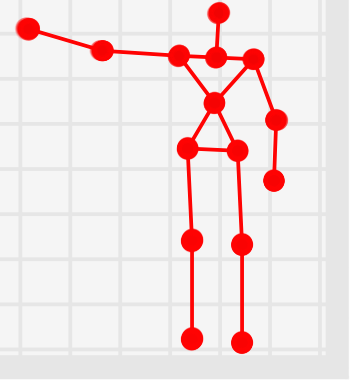
\includegraphics[width=4cm]{Figures/Example1}
\centering
\caption{Example of a 3D representation of the skeleton shape data retrieved from the Kinect \label{fig:ske}}
\end{figure}


A kinect module locates the 3D position of the user's joints, and retrieves set of data representing a “skeleton” shape of the data, such as the one in Figure \ref{fig:ske}. In Chapter \ref{Chapter4}, this process will be further explained.

After the trained is finished, the system is able to detect when the new users are posing in a different way than the previous users, and it will be able to learn that novel pose.

\section{Objectives}

The aim of this Thesis is to design a system that is able to:


\begin{description}

  \item[Distinguish between what is known and what is strange] \hfill \newline
The system will have to identify when a new entry of data is different from anything known before and alert about it. If the entry is detected as already known or not interesting, the program will have to ignore it. It is important to highlight that we cannot consider a \emph{right} way of posing, but a \emph{learned} way of posing. New instances will be tested against these \emph{learned} instances.

\clearpage
  \item[Identify when an entry is interesting] \hfill \\
If, in the example opening the thesis, we asked our friend about any new move he does, we would bother him. If he scratches his arm, or drops the pencil or stretches, all this moves will be strange to us, but if we ask him every time 'What are you doing?' he would think that we are crazy. We are not interested in asking him unless the event has happened frequently enough to be interesting.

To imitate human behavior, the system will have to distinguish between when a new entry is detected as different because it is noise, meaning that the camera was not able to record it properly, it was a one-time event, or because it is a novel entry.

  \item[Learn from novel data] \hfill \\
The system, after detecting a novel entry, will have to add it to its knowledge base. Thus, a mechanism needs to be established to incorporate these interesting and strange entries in a continuous way. 

The detection of novel poses is the main objective of the Thesis, implying that the system will need to be able to alert the user of this event, so that we can check that the system is operating correctly. After alerting, the system can ask the user 'What are you doing?' or whatever the experiment require. 

\item[Aim to have a high detection rate while keeping the false alarm rate low] \hfill \\
  The program will aim to identify as many novel entries as possible, while ignoring as many known or uninteresting entries as possible. This means that the program has to avoid false alarms, so it will not bother the interacting user unnecessarily. 

  \item[Have an autonomous behavior and display information] \hfill \\
The system will need to do this active learning tasks autonomously. To check the correct operation of the system, some kind of user interface will need to be built to display the system information, such as when a new pose is detected as novel.

While establishing a human-robot, visual or voice, interaction is out of the scope of this Thesis, we will need to define mechanisms that allow our system to transmit information to other interaction modules created by the research group where this Thesis was developed. This implies creating an alert system that can transmit this information.  


\end{description}

\clearpage
\section{Organization, structure of the document}

This document is organized as follows. Chapter \ref{Chapter2} introduces the formal definition of the problem and the machine learning algorithms used to address it. Chapter \ref{Chapter3} describes proposed solution as the software architecture and is followed by the results of the testing of the software with real data in different experiments in Chapter \ref{Chapter4}. Chapter \ref{Chapter5} presents an overview of the methods an approaches used in related work. Finally, Chapter \ref{Chapter6} summarizes the main contributions and describes future work and opened issues worth studying.

\begin{flushright}

\end{flushright}
